%============================================================================
%  Telaria — Presentación de defensa do TFG
%  Estrutura baseada en guion-largo.md
%  Compilar con: pdflatex (dúas pasadas) ou latexmk -pdf presentacion.tex
%============================================================================
\documentclass[11pt,aspectratio=169]{beamer}

\usepackage[T1]{fontenc}
\usepackage[utf8]{inputenc}
\usepackage[galician]{babel}
\usepackage{graphicx}
\usepackage{booktabs}
\usepackage{tikz}
\usetikzlibrary{shapes.geometric, arrows.meta, positioning, fit, backgrounds}

% Figuras reutilizadas da memoria
\graphicspath{{../memoria/diagrams/}{../memoria/screenshots/}{../memoria/assets/usc/}}

%--------------------------------------------------------------------------
%  Paleta de cores de Telaria (mesma que a memoria)
%--------------------------------------------------------------------------
\definecolor{telPrimary}{HTML}{8b3ce0}
\definecolor{telDeep}{HTML}{3d1e7a}
\definecolor{telTint}{HTML}{7c3aed}
\definecolor{telSecondary}{HTML}{f59e0b}
\definecolor{telWarning}{HTML}{dc2626}
\definecolor{telLbg}{HTML}{f7f3ff}
\definecolor{telLui}{HTML}{ede3fd}
\definecolor{telBorder}{HTML}{d4c2f9}
\definecolor{telInk}{HTML}{2b1440}
\definecolor{telGrey}{HTML}{6b6480}

%--------------------------------------------------------------------------
%  Tema propio (flat, estilo Metropolis) — sen dependencias externas
%--------------------------------------------------------------------------
\usetheme{default}
\usecolortheme{default}
\usefonttheme{professionalfonts}
\setbeamertemplate{navigation symbols}{}
\setbeamertemplate{itemize items}[circle]
\setbeamertemplate{sections/subsections in toc}[circle]

\setbeamercolor{normal text}{fg=telInk, bg=white}
\setbeamercolor{structure}{fg=telPrimary}
\setbeamercolor{alerted text}{fg=telWarning}
\setbeamercolor{frametitle}{fg=white, bg=telPrimary}
\setbeamercolor{title}{fg=telDeep}
\setbeamercolor{itemize item}{fg=telTint}
\setbeamercolor{itemize subitem}{fg=telSecondary}
\setbeamercolor{block title}{fg=white, bg=telTint}
\setbeamercolor{block body}{fg=telInk, bg=telLbg}

\setbeamerfont{frametitle}{series=\bfseries, size=\large}
\setbeamerfont{title}{series=\bfseries, size=\Huge}
\setbeamerfont{block title}{series=\bfseries}

% Barra superior do título de cada diapo
\setbeamertemplate{frametitle}{%
  \nointerlineskip
  \begin{beamercolorbox}[wd=\paperwidth,ht=2.6ex,dp=1.2ex,leftskip=0.6cm,rightskip=0.6cm]{frametitle}%
    \usebeamerfont{frametitle}\insertframetitle%
  \end{beamercolorbox}%
}

% Pé de páxina discreto
\setbeamertemplate{footline}{%
  \hbox{%
    \begin{beamercolorbox}[wd=.5\paperwidth,ht=2.2ex,dp=1ex,leftskip=0.6cm]{}%
      \color{telGrey}\scriptsize Telaria — TFG%
    \end{beamercolorbox}%
    \begin{beamercolorbox}[wd=.5\paperwidth,ht=2.2ex,dp=1ex,rightskip=0.6cm]{}%
      \hfill\color{telGrey}\scriptsize Jorge Otero Pailos \quad \insertframenumber%
    \end{beamercolorbox}%
  }%
}

% Diapositiva de sección (separadores)
\setbeamertemplate{section page}{%
  \begin{centering}
    {\usebeamerfont{title}\color{telPrimary}\insertsectionhead\par}
  \end{centering}
}
\AtBeginSection[]{%
  \begin{frame}[plain,noframenumbering]
    \vfill
    \begin{center}
      {\color{telBorder}\rule{0.28\textwidth}{1.6pt}}\\[0.8em]
      {\usebeamerfont{title}\Large\bfseries\color{telDeep}\insertsectionhead\par}
      \vspace{0.7em}
      {\color{telBorder}\rule{0.28\textwidth}{1.6pt}}
    \end{center}
    \vfill
  \end{frame}
}

% Comando auxiliar: chip/etiqueta destacada
\newcommand{\chip}[1]{\tikz[baseline=(x.base)]{\node[fill=telLui, text=telDeep, rounded corners=3pt, inner sep=3pt, font=\footnotesize\bfseries] (x) {#1};}}

%--------------------------------------------------------------------------
%  Metadatos
%--------------------------------------------------------------------------
\title{Telaria}
\subtitle{Aplicación móbil colaborativa para a xestión integral de viaxes en grupo}
\author{Jorge Otero Pailos}
\institute{Titores: Víctor J. Gallego Fontenla \and Pedro Gamallo Fernández}
\date{Xuño 2026}

\begin{document}

%============================== 1. PORTADA ==================================
\begin{frame}[plain,noframenumbering]
  \vfill
  \begin{center}
    {\color{telPrimary}\rule{0.35\textwidth}{2pt}}\\[1.2em]
    {\usebeamerfont{title}\color{telDeep} Telaria}\\[0.6em]
    {\large\color{telInk} Aplicación móbil colaborativa\\ para a xestión integral de viaxes en grupo}\\[1.6em]
    {\color{telPrimary}\rule{0.35\textwidth}{2pt}}\\[1.6em]
    {\normalsize\bfseries\color{telInk} Jorge Otero Pailos}\\[0.4em]
    {\small\color{telGrey} Titores: Víctor J. Gallego Fontenla \ · \ Pedro Gamallo Fernández}\\[0.8em]
    {\small\color{telGrey} Grao en Enxeñaría Informática \ — \ ETSE · USC \ — \ Xuño 2026}
  \end{center}
  \vfill
\end{frame}

%============================== 2. MOTIVACIÓN ===============================
\begin{frame}{Motivación e problema}
  \centering
  \begin{tikzpicture}[
    logo/.style={inner sep=0pt},
    capt/.style={align=center, text width=3.6cm, font=\scriptsize, text=telInk},
    disp/.style={-{Latex[length=2.2mm]}, telWarning, line width=1pt, dashed, opacity=0.85}]

    % --- Logos nas catro esquinas, coa súa pregunta debaixo ---
    \node[logo] (wa)  at (-5.3, 2.45) {
\includegraphics[height=1.45cm]{assets/whatsapp.png}};
    \node[capt, below=2pt of wa] {\itshape «Avisaches a Laura?»\\ «Pásasme as fotos?»};
    \node[logo] (cal) at ( 5.3, 2.45) {
\includegraphics[height=1.1cm]{assets/gcalendar.png}};
    \node[capt, below=2pt of cal] {\itshape «É hoxe este plan... ou o outro?»};
    \node[logo] (dr)  at (-5.3,-2.15) {
\includegraphics[height=1.1cm]{assets/gdrive.png}};
    \node[capt, below=2pt of dr] {\itshape «Onde están os billetes?»};
    \node[logo] (tri) at ( 5.3,-2.15) {
\includegraphics[height=1.45cm]{assets/tricount.png}};
    \node[capt, below=2pt of tri] {\itshape «Quen pagou a comida? A quen lle debo cartos?»};

    % --- Texto central: só a primeira e a última frase ---
    \node[align=center, text width=6.4cm, text=telInk] (txt) at (0,0) {%
      {\bfseries\color{telDeep} Organizar unha viaxe en grupo é un caos disperso}\\[10pt]
      {\small Cada parte organízase por separado e a información acaba \textbf{espallada —e ás veces pérdese—} entre apps distintas:}};

    % --- Frechas: a información dispérsase cara a cada app ---
    \draw[disp] (txt.north west) to[bend left=8]  (wa.east);
    \draw[disp] (txt.north east) to[bend right=8] (cal.west);
    \draw[disp] (txt.south west) to[bend right=8] (dr.east);
    \draw[disp] (txt.south east) to[bend left=8]  (tri.west);
  \end{tikzpicture}
\end{frame}

%============================== 3. SOLUCIÓN =================================
\begin{frame}{Solución e diferenciación}
  \textbf{Telaria integra nun só lugar todo o que precisa unha viaxe en grupo,} aforrando esforzo e previndo erros:
  \medskip
  \begin{columns}[c]
    \begin{column}{0.5\textwidth}
      \centering
      \begin{tikzpicture}[
        mod/.style={draw=telBorder, line width=0.9pt, fill=telLui, text=telDeep,
                    rounded corners=6pt, align=center, font=\footnotesize\bfseries,
                    inner sep=3.5pt, text width=1.85cm, minimum height=0.72cm},
        hub/.style={ellipse, fill=telPrimary, text=white, font=\normalsize\bfseries, inner sep=5pt},
        rama/.style={telGrey, line width=1pt}]
        \def\R{2.2cm}
        \node[hub] (T) at (0,0) {Telaria};
        \node[mod] (m1) at (90:\R)  {Ciclo de vida da viaxe};
        \node[mod] (m2) at (141:\R) {Gastos e liquidacións};
        \node[mod] (m3) at (193:\R) {Eventos e calendario};
        \node[mod] (m4) at (244:\R) {Documentos compartidos};
        \node[mod] (m5) at (296:\R) {Chat de grupo};
        \node[mod] (m6) at (347:\R) {Asistente de IA};
        \node[mod] (m7) at (38:\R)  {Rede de amizades};
        \begin{scope}[on background layer]
          \foreach \m in {m1,m2,m3,m4,m5,m6,m7} \draw[rama] (T) -- (\m);
        \end{scope}
      \end{tikzpicture}
    \end{column}
    \begin{column}{0.5\textwidth}
      \begin{block}{Ademais}
        \begin{itemize}
          \item Todo \textbf{nunha soa aplicación}, pensada para viaxes en grupo
          \item \textbf{Sen ``organizador''}: todos os membros teñen as mesmas capacidades, evitando atrancos e dependencias dunha soa persoa
        \end{itemize}
      \end{block}
    \end{column}
  \end{columns}
  \vspace{0.6em}
  \centering\small\color{telGrey} Obxectivo: unha app móbil multiplataforma que resolva a fragmentación nun único espazo colaborativo.
\end{frame}

%============================== 4. ARQUITECTURA =============================
\begin{frame}{Arquitectura xeral}
  \begin{center}
    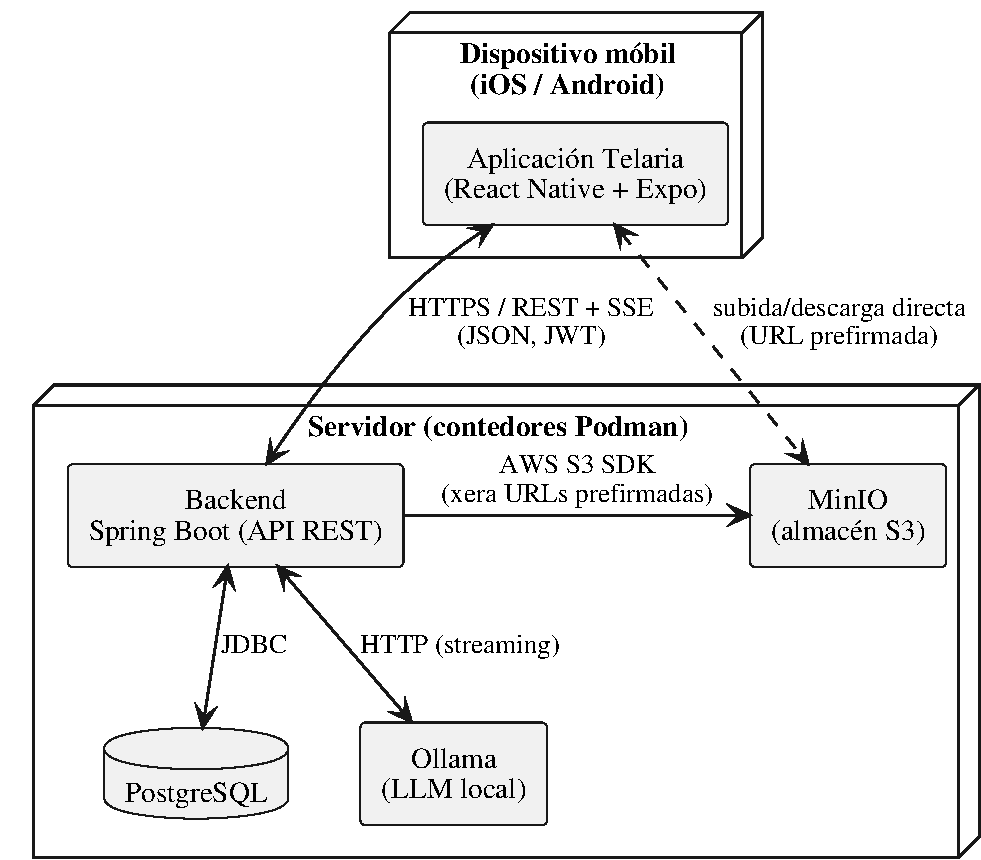
\includegraphics[width=0.98\textwidth]{arquitectura.pdf}
  \end{center}
  \vspace{-0.2em}
  \begin{columns}[T]
    \begin{column}{0.5\textwidth}
      \small
      \textbf{Cliente-servidor}, porque hai datos compartidos en tempo real (gastos, eventos, chat) que deben estar sincronizados e consistentes para todos.
    \end{column}
    \begin{column}{0.5\textwidth}
      \small
      \textbf{Cliente:} app móbil multiplataforma (React Native + Expo).\\
      \textbf{Servidor}: Spring Boot + (contedores)PostgreSQL + MinIO (S3) + Ollama.\\
      Enfoque \textbf{API-first}: OpenAPI é o contrato que se escribe primeiro.
    \end{column}
  \end{columns}
\end{frame}

%============================== 6. DECISIÓNS TÉCNICAS =======================

% --- 6.0 Elección de tecnoloxías ---
\begin{frame}{Decisións técnicas · Elección de tecnoloxías (1/6)}
  \small
  \renewcommand{\arraystretch}{1.4}
  \begin{center}
  \begin{tabular}{@{}l p{8.4cm}@{}}
    \toprule
    {\bfseries\color{telDeep}Tecnoloxía} & {\bfseries\color{telDeep}Por que a escollemos} \\
    \midrule
    {\bfseries\color{telTint}React Native + Expo} & Cliente \textbf{iOS e Android} cunha soa base de código TypeScript; Expo simplifica o \textit{build} e o acceso ás APIs nativas. \\
    {\bfseries\color{telTint}Spring Boot} & Ecosistema \textbf{Java} maduro: inxección de dependencias, seguridade e integración natural coa xeración de código \textbf{OpenAPI}. \\
    {\bfseries\color{telTint}PostgreSQL} & Base relacional \textbf{ACID}, idónea para datos moi relacionados (viaxes, membros, gastos) con integridade referencial. \\
    {\bfseries\color{telTint}MinIO} & Almacén de obxectos \textbf{compatible con S3} e autohospedable: documentos fóra da BD e migración a S3 \textbf{sen tocar código}. \\
    {\bfseries\color{telTint}Ollama} & \textbf{LLM en local}: privacidade, sen custos de APIs externas e API REST estándar que serve calquera modelo. \\
    \bottomrule
  \end{tabular}
  \end{center}
\end{frame}

% --- 6.1 API-first / OpenAPI (logo oficial) ---
\begin{frame}{Decisións técnicas · API-first con OpenAPI (2/6)}
  \begin{columns}[c]
    \begin{column}{0.44\textwidth}
      \centering
      
\includegraphics[width=0.92\textwidth]{assets/openapi-logo.png}
    \end{column}
    \begin{column}{0.56\textwidth}
      \textbf{Por que}
      \begin{itemize}\small
        \item O contrato OpenAPI escríbese \textbf{primeiro}: única fonte de verdade.
        \item A partir del \textbf{xérase código} nos dous extremos: interfaces e DTOs no backend, tipos TypeScript no frontend.
        \item Calquera incoherencia salta en \textbf{tempo de compilación}, non en produción.
        \item Ademais: documentación viva (Swagger UI).
      \end{itemize}
    \end{column}
  \end{columns}
\end{frame}

% --- 6.2 Autenticación: access JWT + refresh opaco ---
\begin{frame}{Decisións técnicas · Autenticación: JWT + refresh opaco (3/6)}
  \begin{columns}[c]
    \begin{column}{0.52\textwidth}
      \centering
      \resizebox{\linewidth}{!}{%
      \begin{tikzpicture}[font=\footnotesize,
        card/.style={draw=telBorder, line width=0.9pt, rounded corners=5pt, fill=telLbg, text=telInk, align=left, inner sep=7pt, text width=4.6cm}]
        \node[card] (acc) {{\bfseries\color{telDeep} Access token · JWT}\\[3pt]
          \textbullet~En \textbf{cada petición} (moi frecuente)\\
          \textbullet~Validado pola \textbf{sinatura} RSA\\
          \textbullet~\textbf{Sen tocar a BD} → \textit{stateless}};
        \node[card, draw=telPrimary, line width=1.1pt, fill=telLui, below=0.45cm of acc] (ref) {{\bfseries\color{telDeep} Refresh token · opaco}\\[3pt]
          \textbullet~Só \textbf{ao renovar} (pouco frecuente)\\
          \textbullet~Cadea aleatoria \textbf{gardada na BD}\\
          \textbullet~Por iso \textbf{pódese invalidar}};
      \end{tikzpicture}}
    \end{column}
    \begin{column}{0.48\textwidth}
      \textbf{Por que}
      \begin{itemize}\small
        \item O \textit{access token} úsase constantemente → interésanos validalo \textbf{sen consultar a BD} (rápido e escalable). Como JWT asinado, \textbf{non se pode revogar}.
        \item O \textit{refresh token} úsase \textbf{poucas veces} (só cando caduca o access), así que o custo de ir á BD é irrelevante.
        \item Por iso faise \textbf{opaco e gardado no servidor}: permite \textbf{invalidalo} (peche de sesión, cambio de contrasinal), imposíbel cun JWT.
      \end{itemize}
    \end{column}
  \end{columns}
\end{frame}

% --- 6.3 SSE chat (hub simplificado) ---
\begin{frame}{Decisións técnicas · Chat en tempo real con SSE (4/6)}
  \begin{columns}[c]
    \begin{column}{0.6\textwidth}
      \centering
      \resizebox{\linewidth}{!}{%
      \begin{tikzpicture}[font=\footnotesize,
        srv/.style={draw=telPrimary, line width=1pt, fill=telLui, rounded corners=5pt, text=telDeep, align=center, inner sep=8pt, font=\bfseries},
        cli/.style={draw=telBorder, fill=white, rounded corners=4pt, text=telInk, align=center, inner sep=4pt, minimum width=1.7cm},
        sub/.style={-{Latex[length=2mm]}, telTint, line width=1pt, dashed},
        snd/.style={-{Latex[length=2mm]}, telSecondary, line width=1.2pt}]
        \node[srv] (s) {Servidor};
        \node[cli, above left=0.7cm and 2.3cm of s] (a) {Membro A};
        \node[cli, left=2.7cm of s] (b) {Membro B};
        \node[cli, below left=0.7cm and 2.3cm of s] (c) {Membro C};
        \node[draw=telBorder, fill=telLbg, cylinder, shape border rotate=90, aspect=0.3, minimum height=0.9cm, minimum width=0.9cm, text=telInk, right=1.5cm of s] (db) {BD};
        \draw[snd] (b) -- node[above, font=\scriptsize, text=telSecondary]{envía} (s);
        \draw[sub] (s) -- node[above, font=\scriptsize, text=telTint]{SSE} (a);
        \draw[sub] (s) -- node[below, font=\scriptsize, text=telTint]{SSE} (c);
        \draw[-{Latex[length=1.5mm]}, telGrey] (s) -- node[above, font=\scriptsize, text=telGrey]{persiste} (db);
      \end{tikzpicture}}
    \end{column}
    \begin{column}{0.4\textwidth}
      \textbf{Por que SSE}
      \begin{itemize}\small
        \item Só fai falta un fluxo \textbf{unidireccional} servidor$\to$cliente.
        \item Máis simple que WebSockets (bidireccional), que aquí sobra.
        \item O servidor \textbf{persiste} a mensaxe e \textbf{difúndea} ao instante a todos os subscritores.
      \end{itemize}
    \end{column}
  \end{columns}
\end{frame}

% --- 6.4 URLs prefirmadas (simplificado) ---
\begin{frame}{Decisións técnicas · URLs prefirmadas (5/6)}
  \begin{columns}[c]
    \begin{column}{0.6\textwidth}
      \centering
      \resizebox{\linewidth}{!}{%
      \begin{tikzpicture}[font=\footnotesize,
        cli/.style={draw=telBorder, fill=white, rounded corners=4pt, text=telInk, align=center, inner sep=6pt, minimum width=1.8cm},
        be/.style={draw=telPrimary, line width=1pt, fill=telLui, rounded corners=5pt, text=telDeep, align=center, inner sep=6pt, font=\bfseries},
        store/.style={draw=telBorder, fill=telLbg, cylinder, shape border rotate=90, aspect=0.3, minimum height=1.2cm, minimum width=1.2cm, text=telInk},
        ctrl/.style={-{Latex[length=2mm]}, telTint, line width=1pt},
        bytes/.style={-{Latex[length=2.5mm]}, telSecondary, line width=1.6pt}]
        \node[cli] (cli) {Cliente};
        \node[be, above right=1.3cm and 1.1cm of cli] (be) {Backend};
        \node[store, right=4.6cm of cli] (mn) {MinIO};
        \draw[ctrl] (cli) to[bend left=18] node[sloped, above, font=\scriptsize]{1. pide subir} (be);
        \draw[ctrl] (be) to[bend left=18] node[sloped, below, font=\scriptsize]{2. URL asinada} (cli);
        \draw[bytes] (cli) -- node[below, font=\scriptsize\bfseries, text=telSecondary]{3. sobe o ficheiro (bytes, directo)} (mn);
      \end{tikzpicture}}
    \end{column}
    \begin{column}{0.4\textwidth}
      \textbf{Por que}
      \begin{itemize}\small
        \item Os \textbf{bytes non pasan polo backend}: el só emite unha URL temporal asinada.
        \item O cliente sobe/descarga \textbf{directamente} contra MinIO.
        \item Descarga o servidor da transferencia → mellor \textbf{escalabilidade}.
      \end{itemize}
    \end{column}
  \end{columns}
\end{frame}

% --- 6.5 Separación en contedores ---
\begin{frame}{Decisións técnicas · Separación en contedores (6/6)}
  \begin{columns}[c]
    \begin{column}{0.5\textwidth}
      \centering
      \resizebox{\linewidth}{!}{%
      \begin{tikzpicture}[font=\footnotesize,
        be/.style={draw=telPrimary, line width=1pt, fill=telLui, rounded corners=5pt, text=telDeep, align=center, font=\bfseries, minimum width=2.1cm, minimum height=1.1cm},
        svc/.style={draw=telBorder, line width=0.8pt, fill=white, rounded corners=4pt, text=telInk, align=center, minimum width=2.5cm, minimum height=0.9cm},
        arr/.style={-{Latex[length=2mm]}, telTint, line width=1pt}]
        \node[svc] (mn) {\textbf{MinIO}\\{\scriptsize almacén S3}};
        \node[svc, above=0.3cm of mn] (pg) {\textbf{PostgreSQL}\\{\scriptsize persistencia}};
        \node[svc, below=0.3cm of mn] (ol) {\textbf{Ollama}\\{\scriptsize LLM local}};
        \begin{scope}[on background layer]
          \node[draw=telPrimary, line width=1pt, rounded corners=8pt, fill=telLui, inner sep=10pt, fit=(pg)(mn)(ol)] (pod) {};
        \end{scope}
        \node[text=telDeep, font=\bfseries\scriptsize, above=1pt of pod.north] {Contedores (Podman)};
        \node[be, left=2.5cm of mn] (be) {Backend\\{\scriptsize Spring Boot · host}};
        \draw[arr] (be) -- node[sloped, above, font=\scriptsize, text=telGrey]{JDBC} (pg.west);
        \draw[arr] (be) -- node[above, font=\scriptsize, text=telGrey]{S3} (mn.west);
        \draw[arr] (be) -- node[sloped, below, font=\scriptsize, text=telGrey]{REST} (ol.west);
      \end{tikzpicture}}
    \end{column}
    \begin{column}{0.5\textwidth}
      \textbf{Por que}
      \begin{itemize}\small
        \item As dependencias —\textbf{PostgreSQL, MinIO e Ollama}— corren cada unha no \textbf{seu propio contedor}; o backend execútase no host e conéctase a elas. Illamento e despregamento reproducible cun só \textit{compose}.
        \item Comunícanse por \textbf{APIs ben definidas}: o almacén fala a \textbf{API S3} (estándar → migrable a AWS S3 \textbf{sen tocar código}); a IA, a \textbf{API REST de Ollama}, que serve calquera modelo local.
        \item Resultado: \textbf{sen vendor lock-in}. Execución local hoxe, portable mañá.
      \end{itemize}
    \end{column}
  \end{columns}
\end{frame}

%============================== 7. UI/UX ===================================
\begin{frame}{Deseño UI/UX e accesibilidade}
  \begin{columns}[c]
    \begin{column}{0.6\textwidth}
      \textbf{Aparencia}
      \begin{itemize}\small
        \item Paleta \textbf{monocromática} centrada no \textbf{violeta}
        \item Vermello reservado para \textbf{accións destrutivas} (eliminar conta, saír da viaxe...)
        \item Tema \textbf{claro e escuro} seleccionable
        \item Tipografía nativa do sistema (coidada e rápida)
      \end{itemize}
      \medskip
      \textbf{Accesibilidade}
      \begin{itemize}\small
        \item Contraste \textbf{WCAG AA}
        \item Etiquetas e \textit{roles} para lectores de pantalla
        \item Respecta o \textbf{movemento reducido} do sistema
        \item Área de pulsación ampliada ao mínimo recomendado
      \end{itemize}
      \medskip
      {\centering
        \colorbox{telDeep}{\rule{1.4em}{0pt}\rule{0pt}{1.1em}}\;
        \colorbox{telPrimary}{\rule{1.4em}{0pt}\rule{0pt}{1.1em}}\;
        \colorbox{telTint}{\rule{1.4em}{0pt}\rule{0pt}{1.1em}}\;
        \colorbox{telLui}{\rule{1.4em}{0pt}\rule{0pt}{1.1em}}\;
        \colorbox{telWarning}{\rule{1.4em}{0pt}\rule{0pt}{1.1em}}\par}
    \end{column}
    \begin{column}{0.4\textwidth}
      \centering
      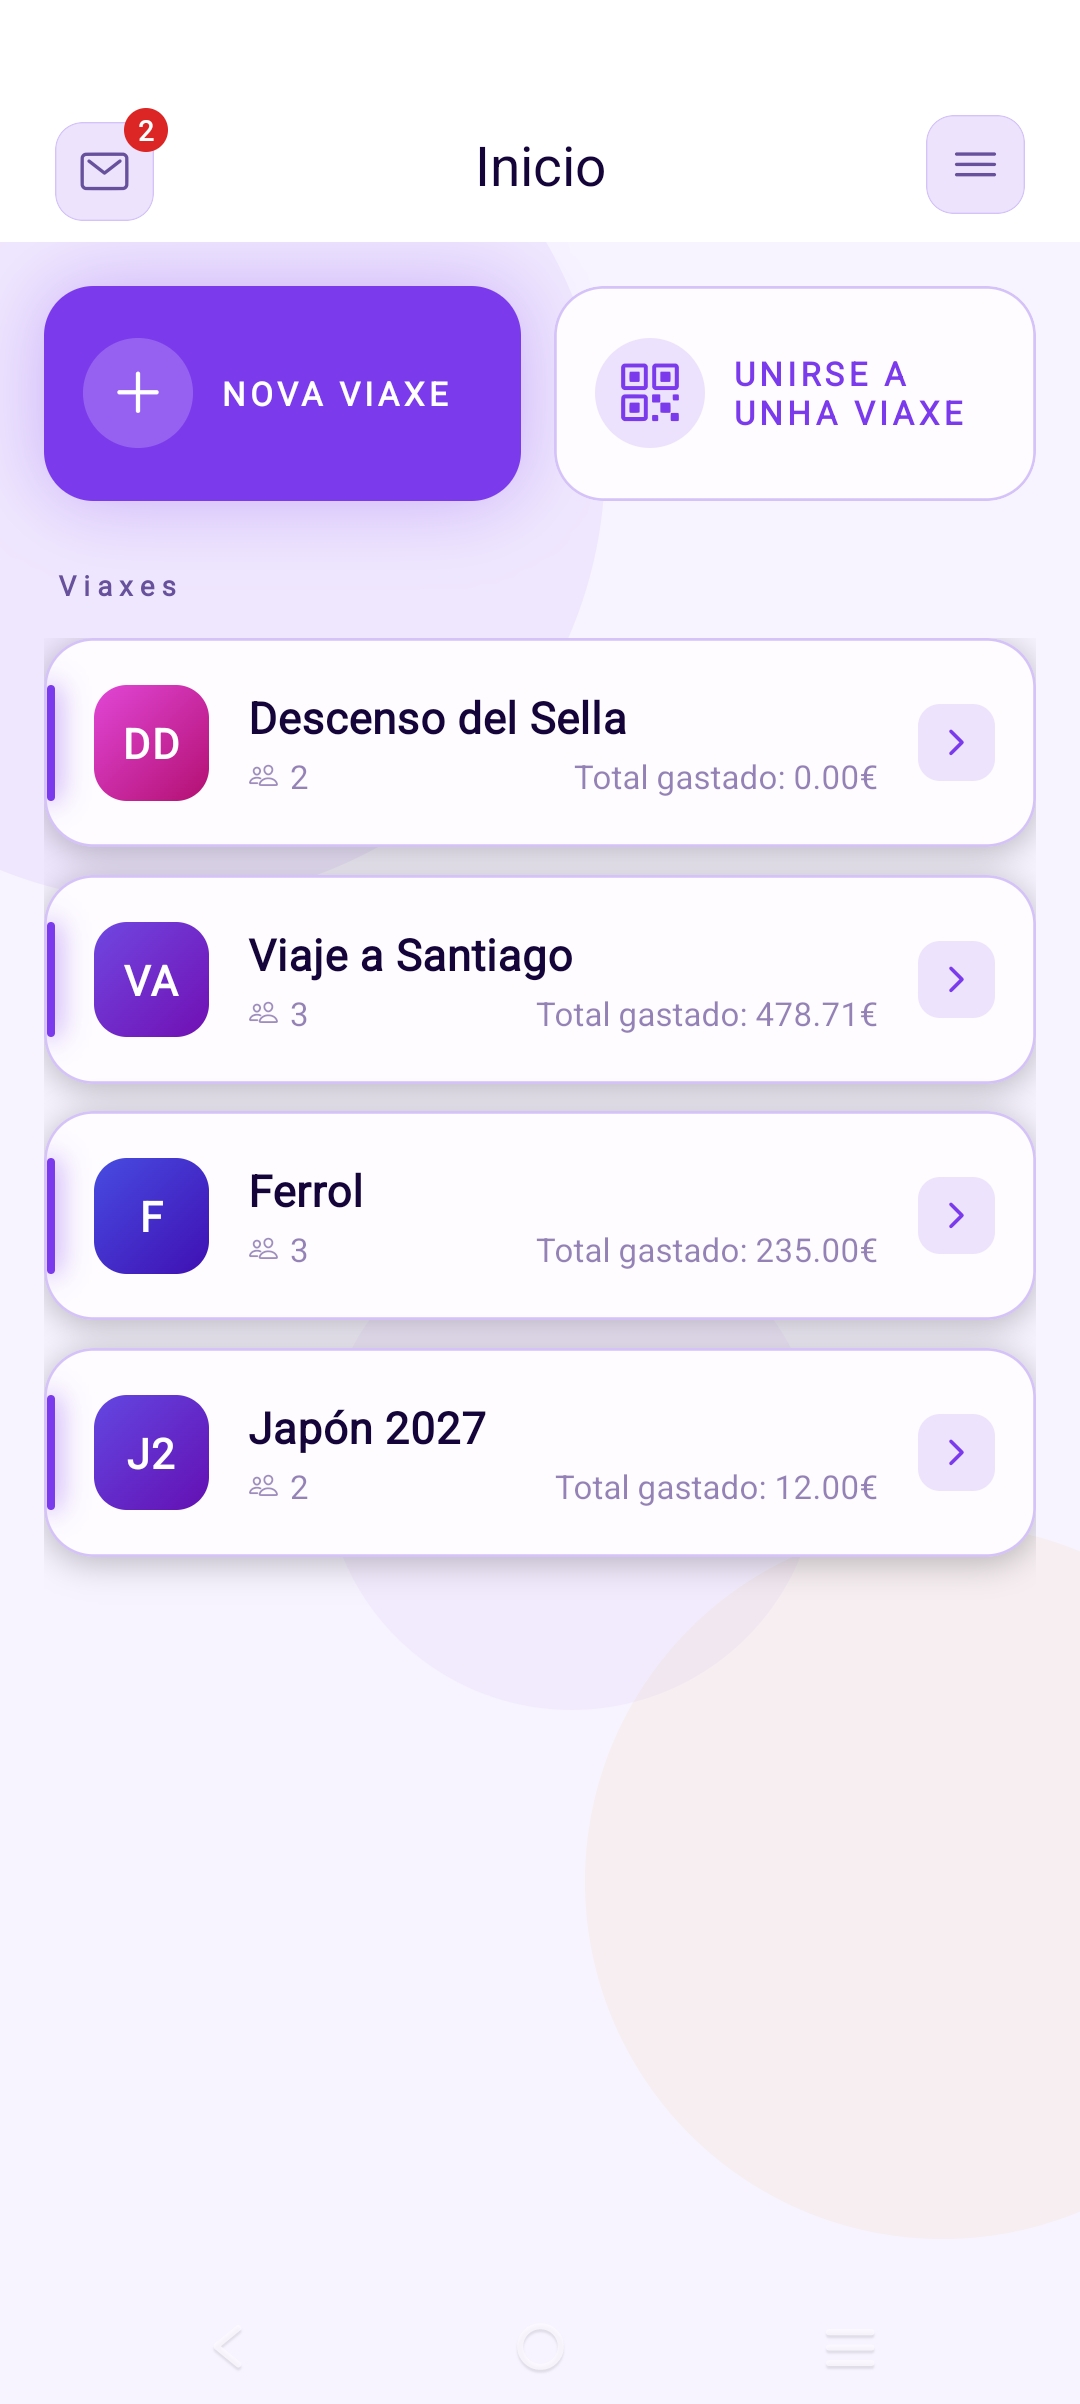
\includegraphics[height=0.78\textheight]{main.jpeg}
    \end{column}
  \end{columns}
\end{frame}

%============================== 8. DEMOSTRACIÓN ============================
\begin{frame}{Demostración}
  \begin{columns}[c]
    \begin{column}{0.5\textwidth}
      \textbf{Percorrido rápido pola aplicación:}
      \begin{enumerate}
        \item Unirse a unha viaxe escaneando un \textbf{código QR}
        \item Rexistrar un gasto → \textbf{recálculo automático} de balances e liquidación suxerida
        \item Crear un evento no calendario cun \textbf{mapa interactivo}
        \item Asistente de \textbf{IA} respondendo en \textit{streaming} co contexto da viaxe
      \end{enumerate}
      \vspace{0.8em}
      \begin{center}
        \chip{$\blacktriangleright$\; Reproducir vídeo da demostración}
      \end{center}
    \end{column}
    \begin{column}{0.5\textwidth}
      \centering
      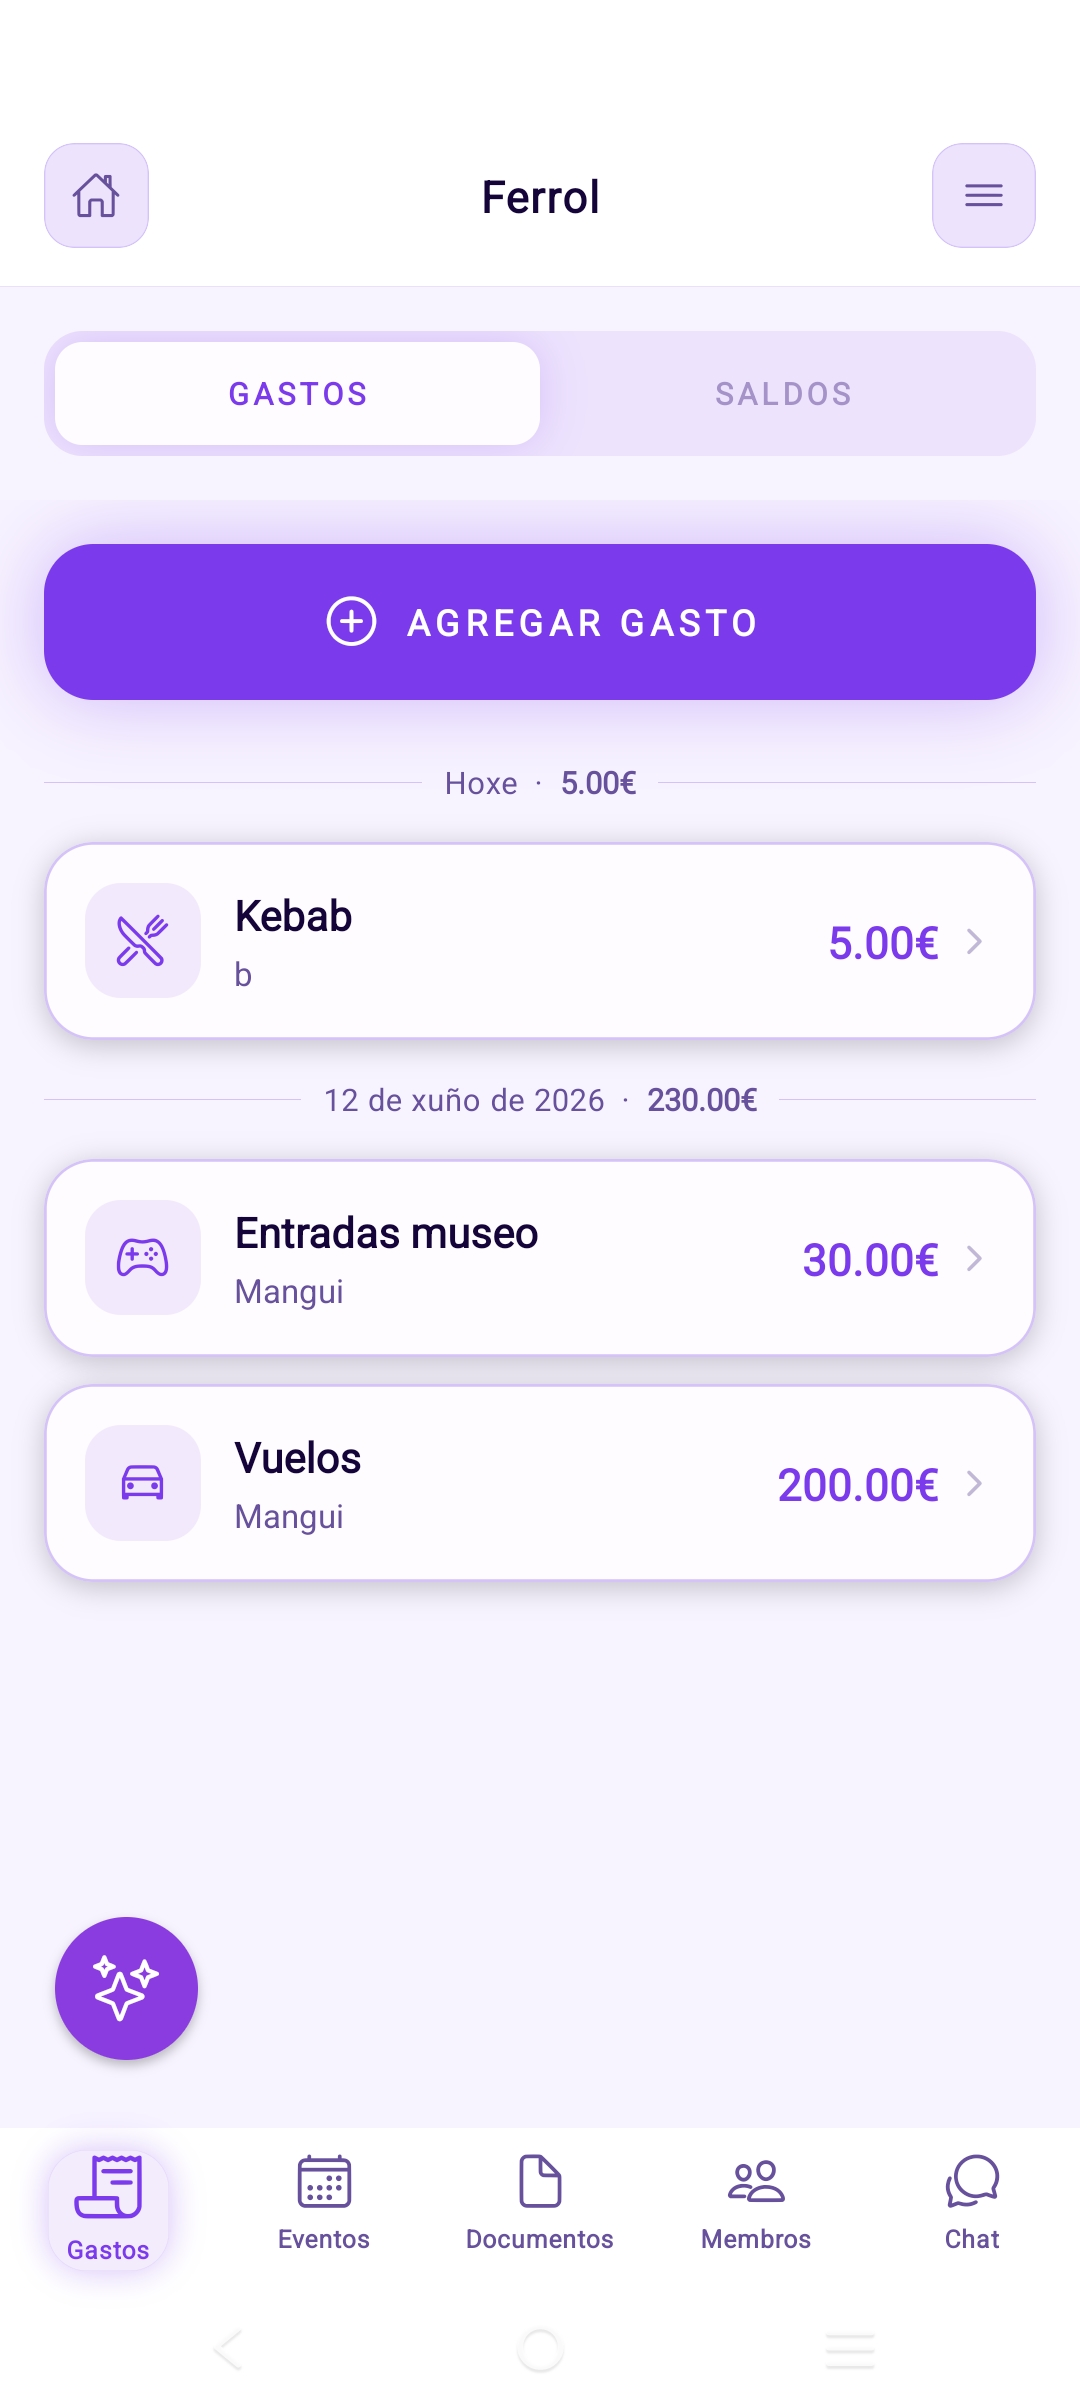
\includegraphics[height=0.72\textheight]{expenses.jpeg}\hspace{0.4em}%
      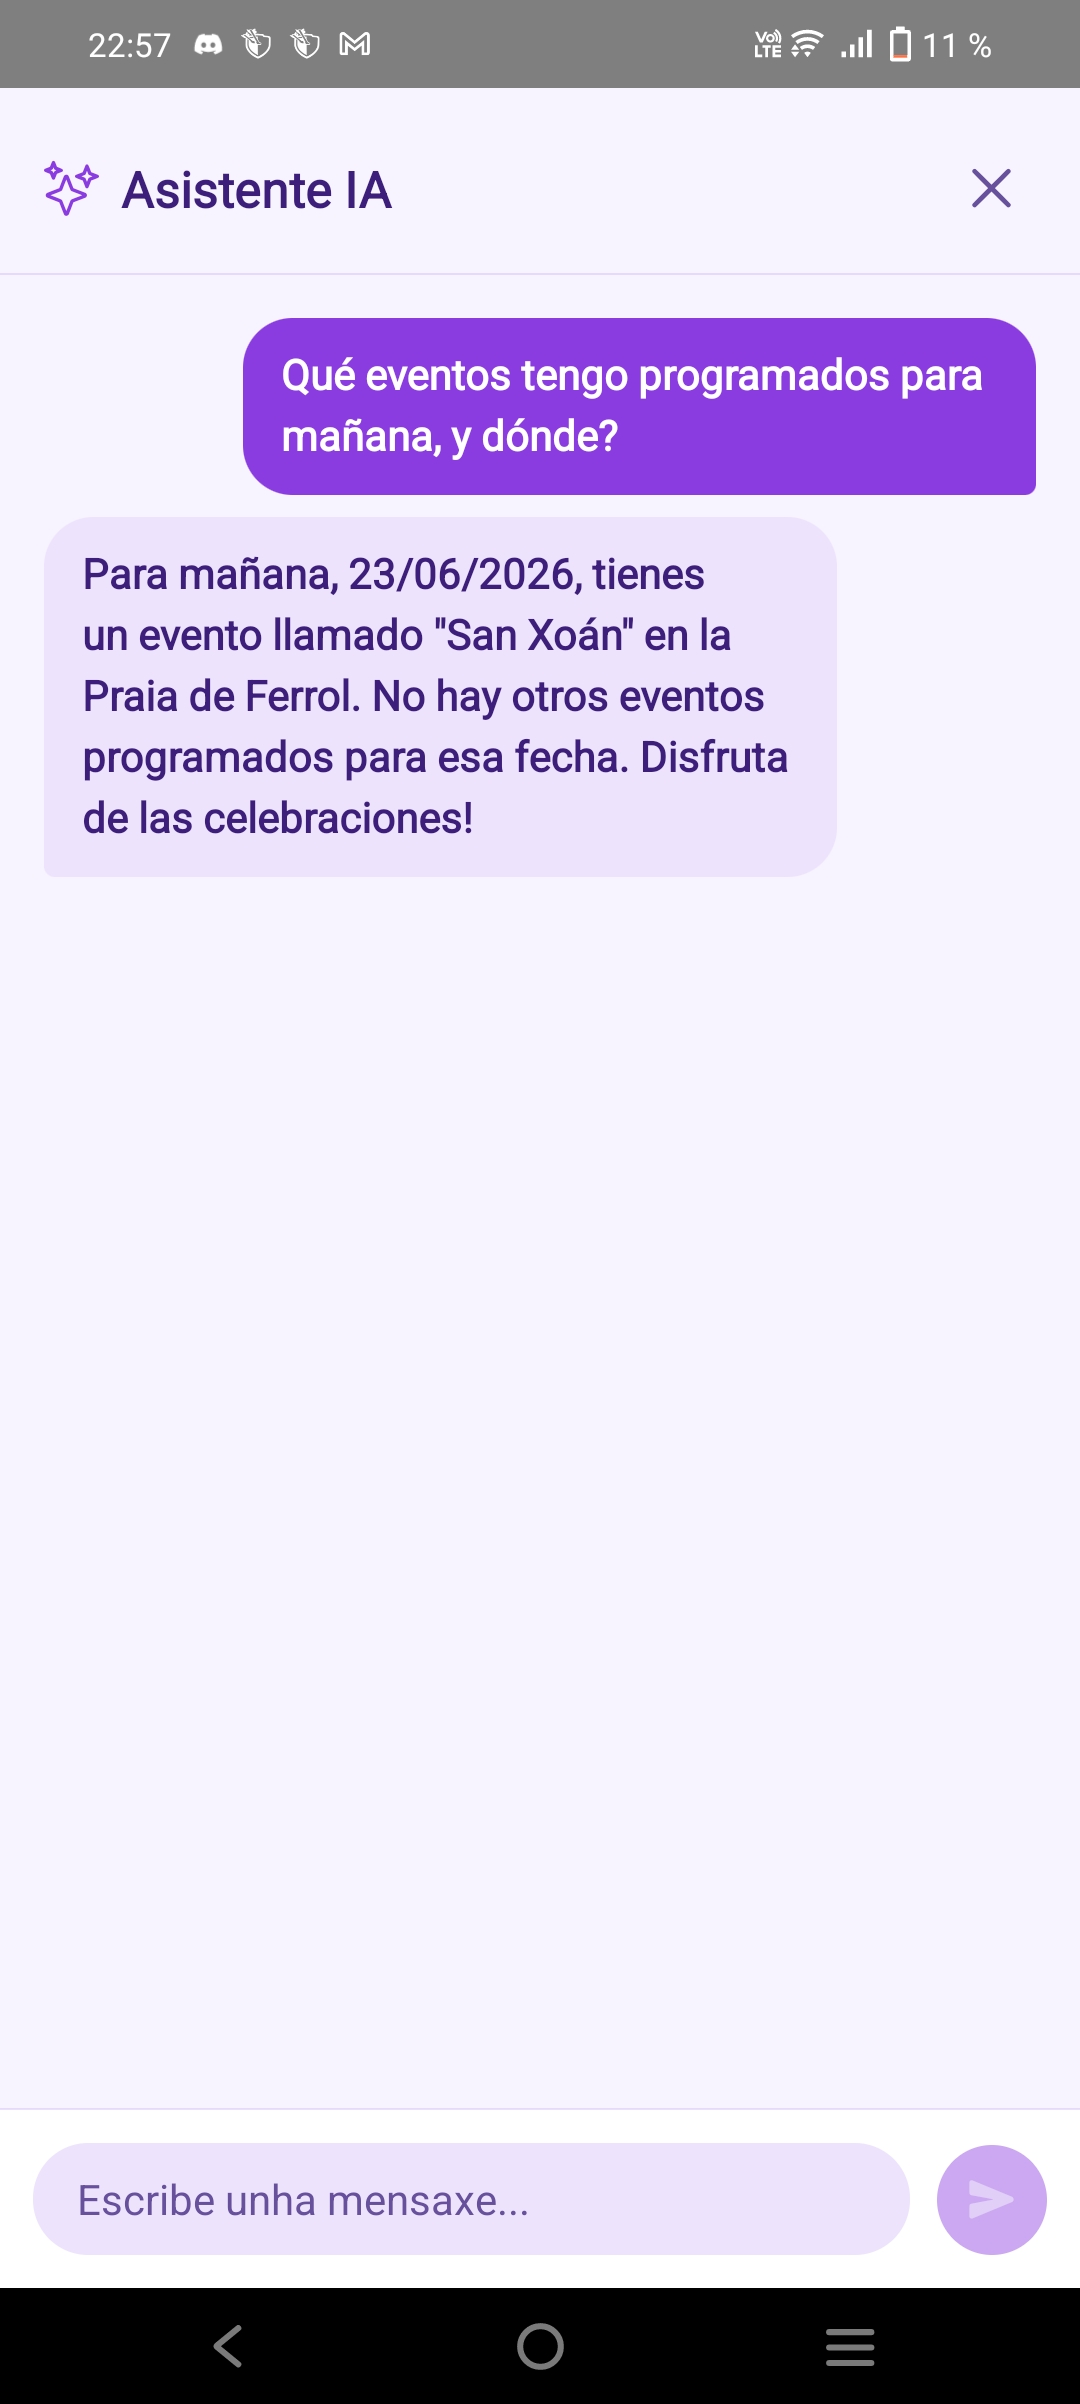
\includegraphics[height=0.72\textheight]{aiChat.jpeg}
    \end{column}
  \end{columns}
\end{frame}

%============================== 9. PROBAS ==================================
\begin{frame}{Probas e resultados}
  \begin{columns}[T]
    \begin{column}{0.46\textwidth}
      \begin{block}{Probas automatizadas: 677}
        \begin{itemize}\small
          \item \textbf{410} no backend (JUnit 5), con integración real contra PostgreSQL e MinIO vía \textbf{Testcontainers}
          \item \textbf{267} no frontend (Jest)
          \item Cobertura do backend \textbf{> 90\%} de liñas
        \end{itemize}
      \end{block}
    \end{column}
    \begin{column}{0.54\textwidth}
      \begin{block}{Avaliación de usabilidade}
        \begin{itemize}\small
          \item Avaliación heurística (10 heurísticas de Nielsen)
          \item \textbf{15 usuarios reais}, protocolo de \textit{pensar en voz alta}, ata a \textbf{saturación}
        \end{itemize}
        \smallskip
        Melloras xa incorporadas:
        \begin{itemize}\small
          \item Acceso aos documentos do día dende o calendario
          \item Ordenación das viaxes por data de creación
          \item Mapa interactivo para escoller a localización dun evento
        \end{itemize}
      \end{block}
    \end{column}
  \end{columns}
\end{frame}

%============================== 10. CONCLUSIÓNS ============================
\begin{frame}{Conclusións}
  \textbf{Os obxectivos cumpríronse na súa totalidade:}
  \medskip
  \begin{itemize}
    \item Telaria \textbf{centraliza} a xestión integral dunha viaxe en grupo nunha soa app.
    \item A arquitectura \textbf{API-first} foi un acerto: mantén sincronizados frontend e backend.
    \item A \textbf{execución local do modelo de linguaxe} evita servizos externos de pago e preserva a privacidade.
  \end{itemize}
  \medskip
  \begin{block}{Principal dificultade técnica}
    Integrar \textbf{Testcontainers} cun entorno de contedores sen \textit{daemon} como \textbf{Podman}.
  \end{block}
\end{frame}

%============================== 11. AMPLIACIÓNS ===========================
\begin{frame}{Ampliacións futuras}
  \begin{itemize}
    \item Notificacións \textbf{push}.
    \item Preparación para \textbf{produción real}: externalizar segredos e habilitar HTTPS.
    \item Integrar as probas do \textbf{frontend} no \textit{pipeline} de integración continua.
    \item Modo \textbf{sen conexión} con sincronización posterior, para destinos con conectividade limitada.
  \end{itemize}
\end{frame}

%============================== 12. PECHE =================================
\begin{frame}[plain,noframenumbering]
  \vfill
  \begin{center}
    {\color{telPrimary}\rule{0.35\textwidth}{2pt}}\\[1.2em]
    {\usebeamerfont{title}\color{telDeep} Grazas pola vosa atención}\\[1em]
    {\large\color{telInk} Quedo á vosa disposición para calquera pregunta.}\\[1.6em]
    {\color{telPrimary}\rule{0.35\textwidth}{2pt}}\\[1.4em]
    {\small\color{telGrey} Jorge Otero Pailos \ — \ Telaria \ — \ TFG · ETSE · USC}
  \end{center}
  \vfill
\end{frame}

\end{document}
